\chapter{Punktesortierung in Schachbrettmustern}
\label{sec:schachbrettAlg} 


Für die reelle Rekonstruktion, wie sie in Kapitel \ref{sec:real} beschrieben wird, sind die korrespondierenden Punkte


In diesem Teil der Masterthesis soll am Ende ein Algorithmus entstehen, welcher durch einen bereits bestehenden Algorithmus zur Detektion von Eckpunkten eines Schachbretts, eine Liste an Eckpunkten bekommt und diese auf deren Nachbarschaftsverhältnisse prüft. Die Schachbretter können dabei sowohl Kissen- als auch Tonnennverzeichnungen aufweisen und oder perspektivisch verzerrt sein. Mit den Algorithmus sollen Punkte wissen in welchen Reihen sie sich sowohl in x- als auch y-Richtung befinden. Jeder Punkt bekommt also eine Indexnummer in x-, sowie y-Richtung beziehungsweise in unserem Beispiel wird die y-Koordinate als \textit{j} bezeichnet und die x-Koordinate als \textit{i}, zugewiesen. Jeder Punkt bekommt mit Hilfe von den Mathematica eigenen \textit{Associations} einen \textit{Key} mit \textit{NeighbourJ} und \textit{NeighbourI} zugeteilt. Mit Hilfe dieser \textit{Keys} kann dann später bei einem Stereobildpaar zum Beispiel die Korrespondierenden Eckpunkte der Schachbretter rausgesucht werden, was vielleicht genauere Ergebnisse liefert also die Suche von Hand. Des weiteren kann dieser Algorithmus in späteren Projekten vielleicht bei der Rausrechnung von Verzeichnungen hilfreich sein.\\



\section{Algorithmus}
%
%Dieser Algorithmus nimmt die Liste mit den Koordinaten der Eckpunkte entgegen und sortiert und nummeriert diese Zeilen- und Spaltenweise durch.\\
%
%Jeder Punkt ist somit über zwei Indizes codiert und enthält die Information, in welcher Zeile und in welcher Spalte des Schachbrettmusters er sich befindet.\\
%
%Da nicht immer garantiert ist, dass alle Punkte innerhalb des Schachbretts zuvor gefunden worden, enthält der Sortierungsalgorithmus eine Funktion, in welchem er Lücken des innerhalb ausfindig macht und synthetische Eckpunkte setzt. Diese synthetisch gesetzten Punkte, werden markiert, so dass sie nicht in die Liste der möglichen korrespondierenden Punkte fallen.

Definieren eines äußeren Rahmens um das SChacbrett durch sucher der Minimalsten und maximalsten Punkte sowohl in x- als auch in y-Richtung\\

Zellen werden in kleinere Suchfenster unterteilt\\

Die Suchfenster in x-Richtung werden mit dem Index $j$ gekennzeichnet die Suchfenster in y-Richtung mit werden mit dem Index $i$ bezeichnet. \\

Alle Punkte in der ersten Suchfenster Reihe von $j$ und von $i$ werden als mögliche Startpunkte gekennzeichnet. In Abbildung \ref{fig:7.1} befinden sich die möglichen Startpunkte innerhalb des blauen Bereichs. Die Suche nach einem Startpunkt und auch nach den ersten Punkten in zwei Richtungen vom Startpunkt aus, ist relativ komplex. Der Grund hierfür ist, dass sämtliche Schachbretter wie in \ref{sec:SchachAlgBeispiele} gezeigt, in Betracht gezogen werden müssen. Um Anhand des Algorithmus später korrespondierende Punkte in zwei Aufnahmen des Schachbretts finden kann, sollte gewährleistet sein, dass der Startpunkt immer an der selben Ecke eines Schachbretts platziert wird.\\

Innerhalb der blau gefärbten Fläche wird nach einem Startpunkt gesucht. Die Suche nach einem Startpunkt wird pro $i$- und $j$-Richtung in zwei Abfragen unterteilt. In der ersten Abfrage wird innerhalb der ersten Suchfensterreihe in $i$-Richtung nach dem Punkt mit der kleinsten $i$-Koordinate gesucht.Dieser Punkt wird als möglicher erster Startpunkte in die Variablen $VecI$ gespeichert. Danach wird geprüft ob es innerhalb der ersten Suchfensterreihe in $i$-Richtung einen weiteren Punkt gibt dessen $j$-Koordinate kleiner ist als die des momentan gesetzten Punktes $VecI$, wird ein solcher Punkt gefunden, so wird dieser Punkt als neuer $VecI$ gesetzt, sofern seine $i$-Koordinate nicht größer ist als die des zuvorigen $VecI$ plus einem Pufferwert. Durch den Puffer wird verhindert, dass ein Punkt als $VecI$ gesetzt wird, welcher sich möglicherweise schon in der zweiten Reihe der Schachbrettpunkte befinden würde. In Abbildung \ref{fig:7.1} ist $VecI$ mit als oranger Punkt abgebildet.\\

%\begin{figure}[!htb]
%	\minipage{0.48\textwidth}
%	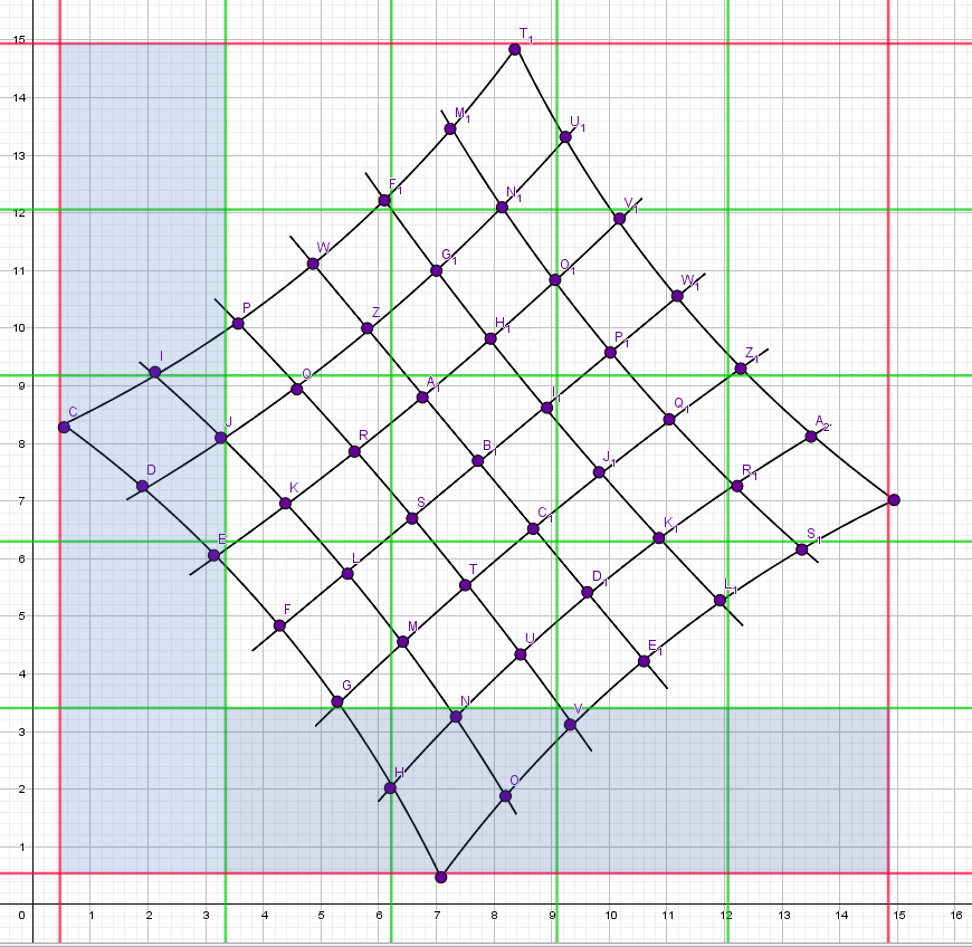
\includegraphics[width=\linewidth]{images/VerzeichnetesSchachbrett_0.png}
%	\caption{ }
%	\label{fig:7.1}
%\end{figure}
%	\endminipage\hfill
\begin{figure}[!htb]
	\centering
	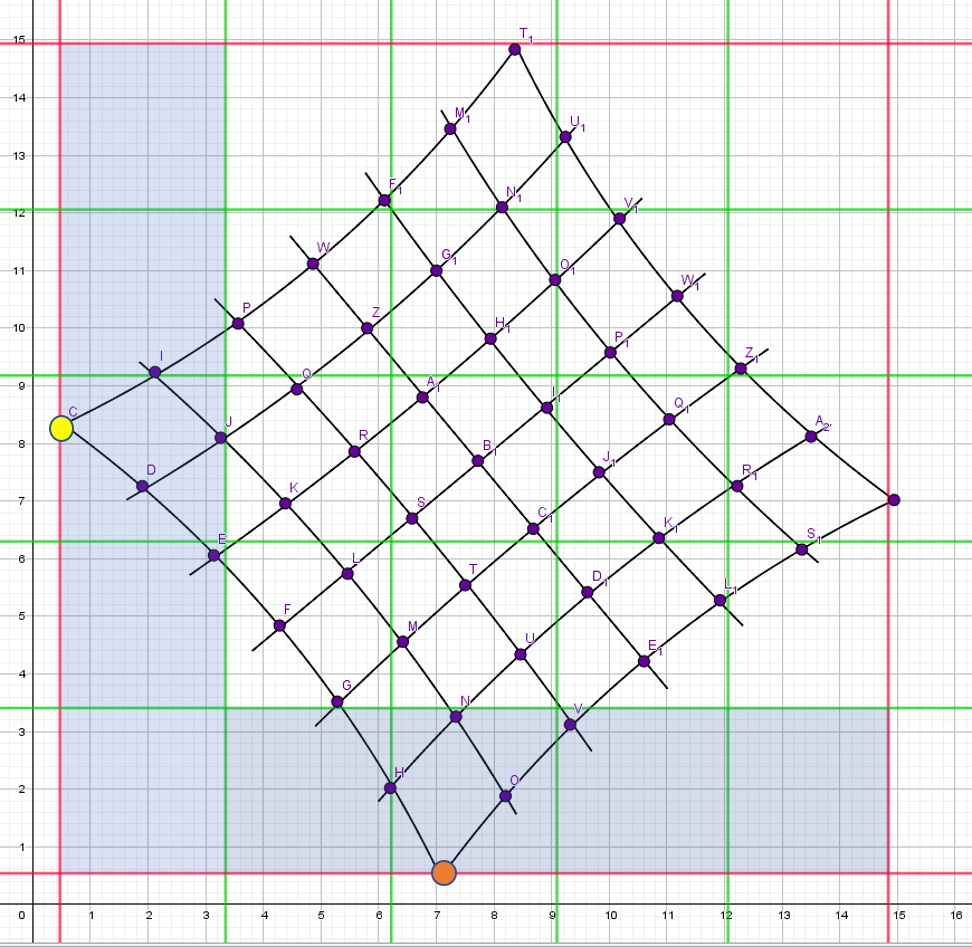
\includegraphics[width=0.8\linewidth]{images/VerzeichnetesSchachbrett_1.png}
	\caption[Startpunktsuche in Schachbrettpunkten]{Die in blau markierten Bereiche beinhalten die möglichen Startpunkte. Der Bereich entlang der horizontalen $j$- Achse bildet die erste Suchfensterreihe in $i$-Richtung. Der blaue Bereich entlang der vertikalen $i$-Achse bildet die erste Suchfensterreihe in $j$-Richtung. Der gelbe Punkt steht für den Punkt welcher als $VecJ$ bezeichnet wurde und der orange Punkt ist derjenige Punkt, welcher als $VecI$ bestimmt wurde}
	\label{fig:7.1}
\end{figure}




Für die Punkte in der ersten Suchfensterreihe in $j$-Richtung wird nach dem Punt mit der 
In der ersten Reihe der Suchfenster in $j$-Richtung wird nach dem Punkt mit der geringsten $j$-Koordinate gesucht.



\begin{figure}[!htb]
	\minipage{0.48\textwidth}
	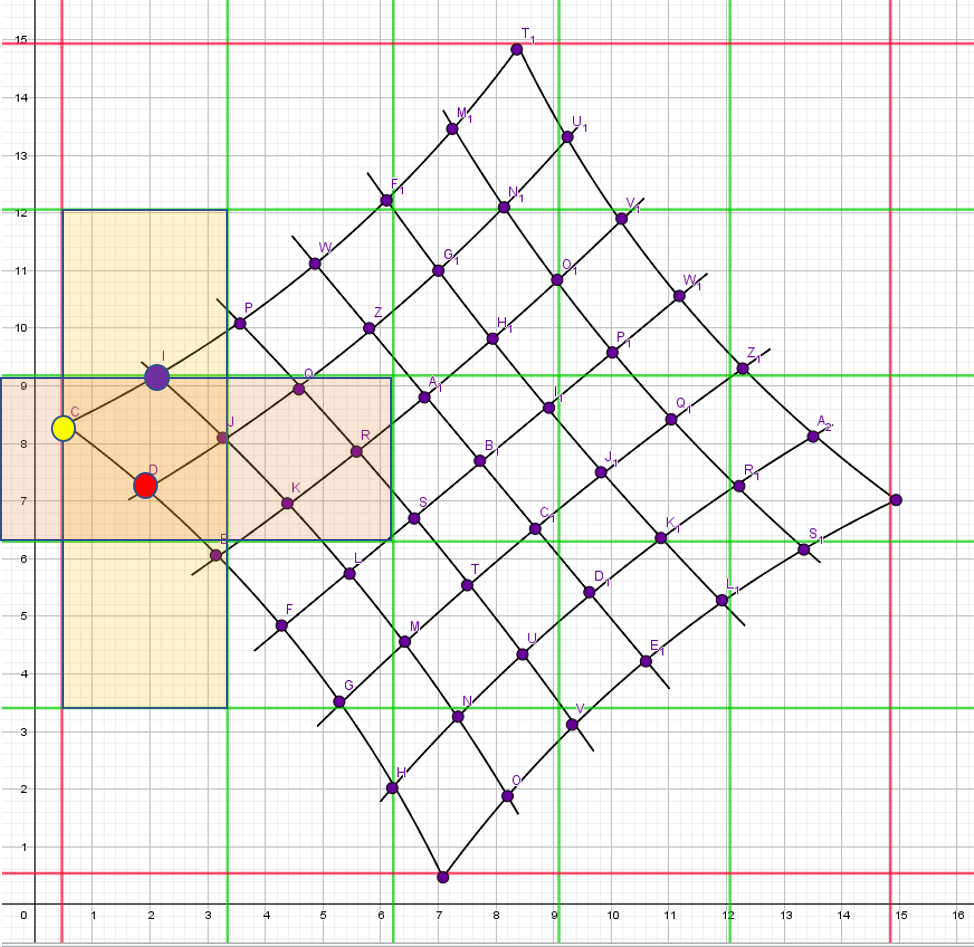
\includegraphics[width=\linewidth]{images/VerzeichnetesSchachbrett_2.png}
	\caption{}
	\label{fig:awesome_image1}
	\endminipage\hfill
	\minipage{0.48\textwidth}
	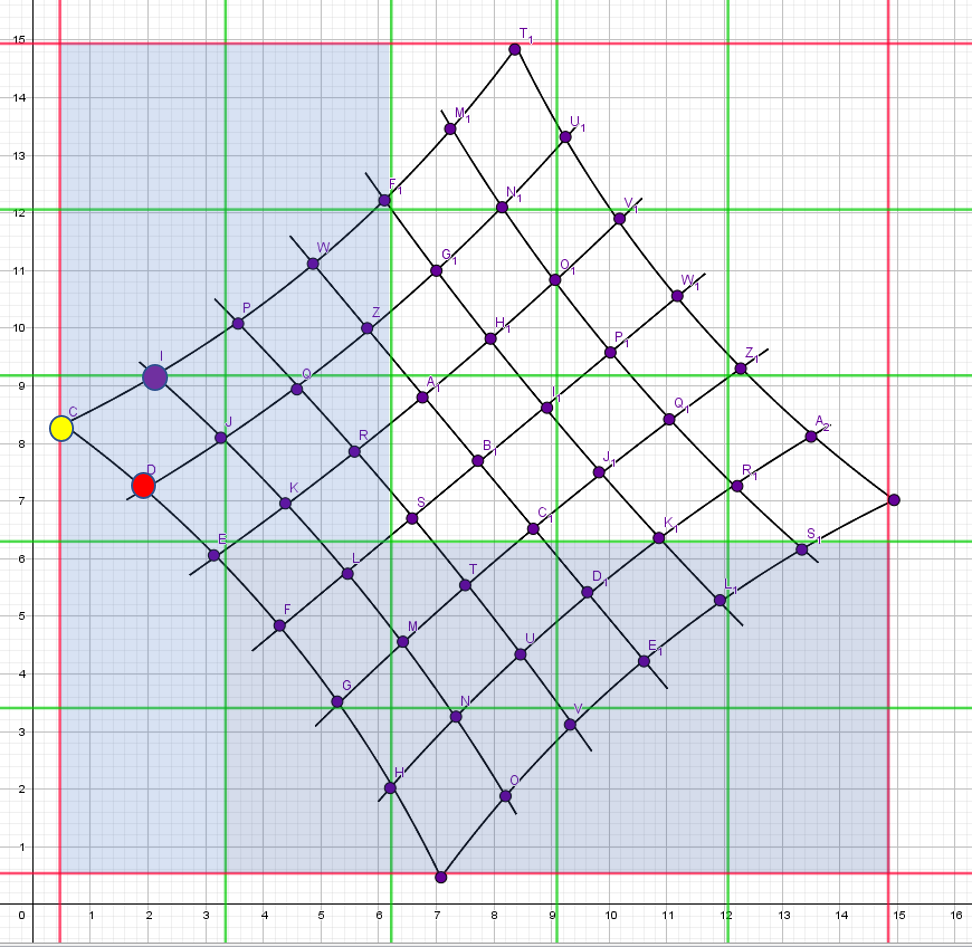
\includegraphics[width=\linewidth]{images/VerzeichnetesSchachbrett_3.png}
	\caption{}
	\label{fig:awesome_image2}
	\endminipage\hfill
	%	\caption{Die mit dem \textit{SURF}-Algorithmus gefundenen Punkte sind mit den gelben Ziffern im Bild gekennzeichnet}
\end{figure}

\begin{minipage}{\linewidth}
	\centering
	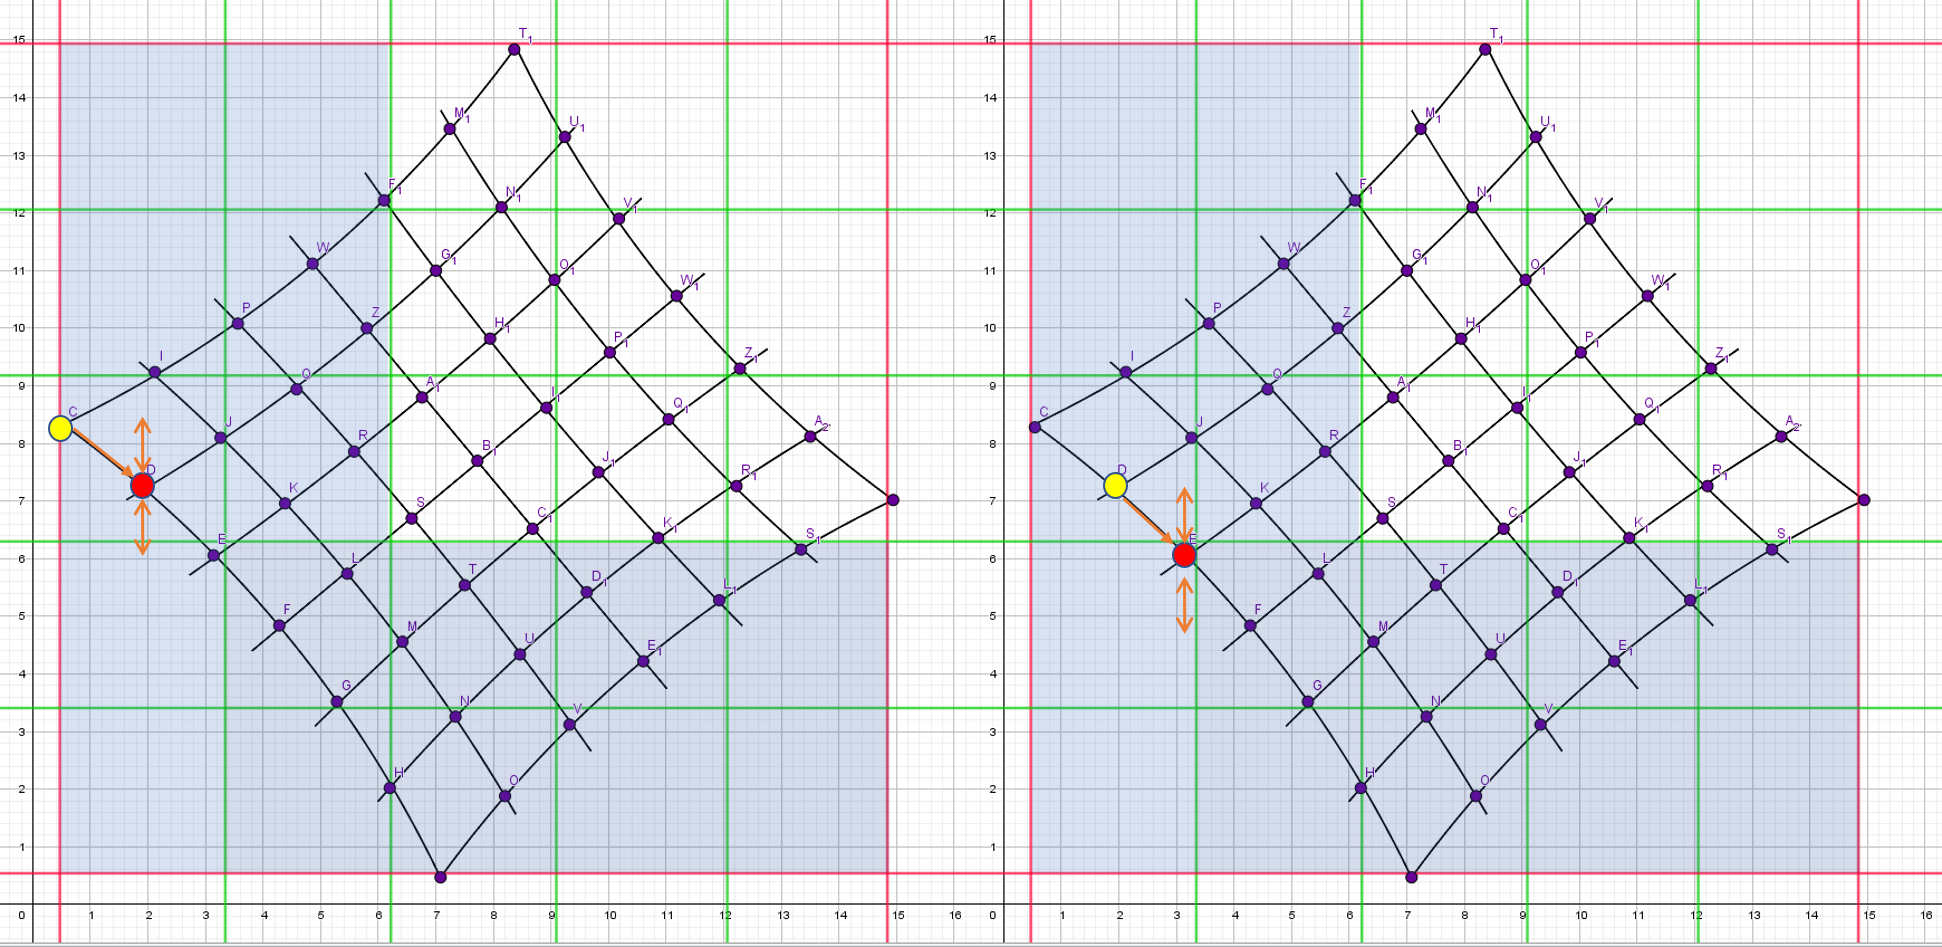
\includegraphics[width=1\linewidth]{images/VerzeichnetesSchachbrett_4.png}
	\captionof{figure}{Klassendiagramm}
\end{minipage}\\

\begin{minipage}{\linewidth}
	\centering
	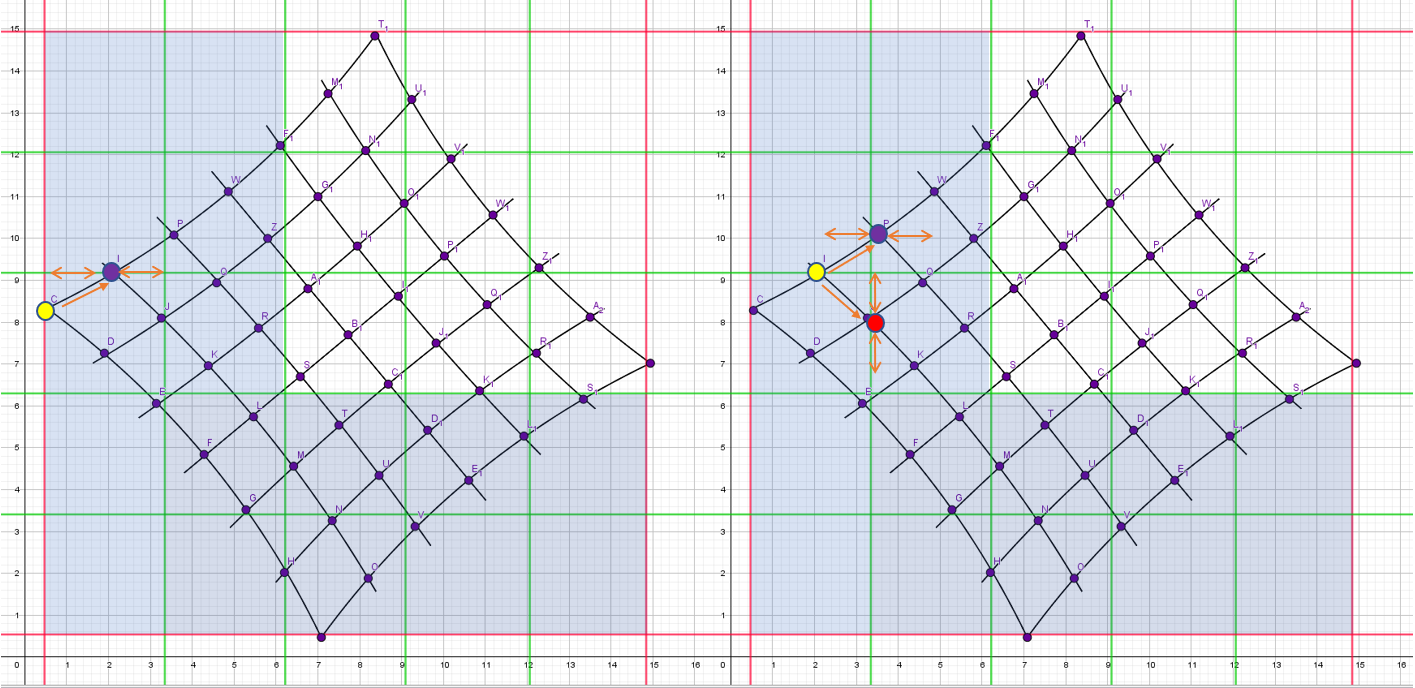
\includegraphics[width=1\linewidth]{images/VerzeichnetesSchachbrett_5.png}
	\captionof{figure}{Klassendiagramm}
\end{minipage}\\

\begin{minipage}{\linewidth}
	\centering
	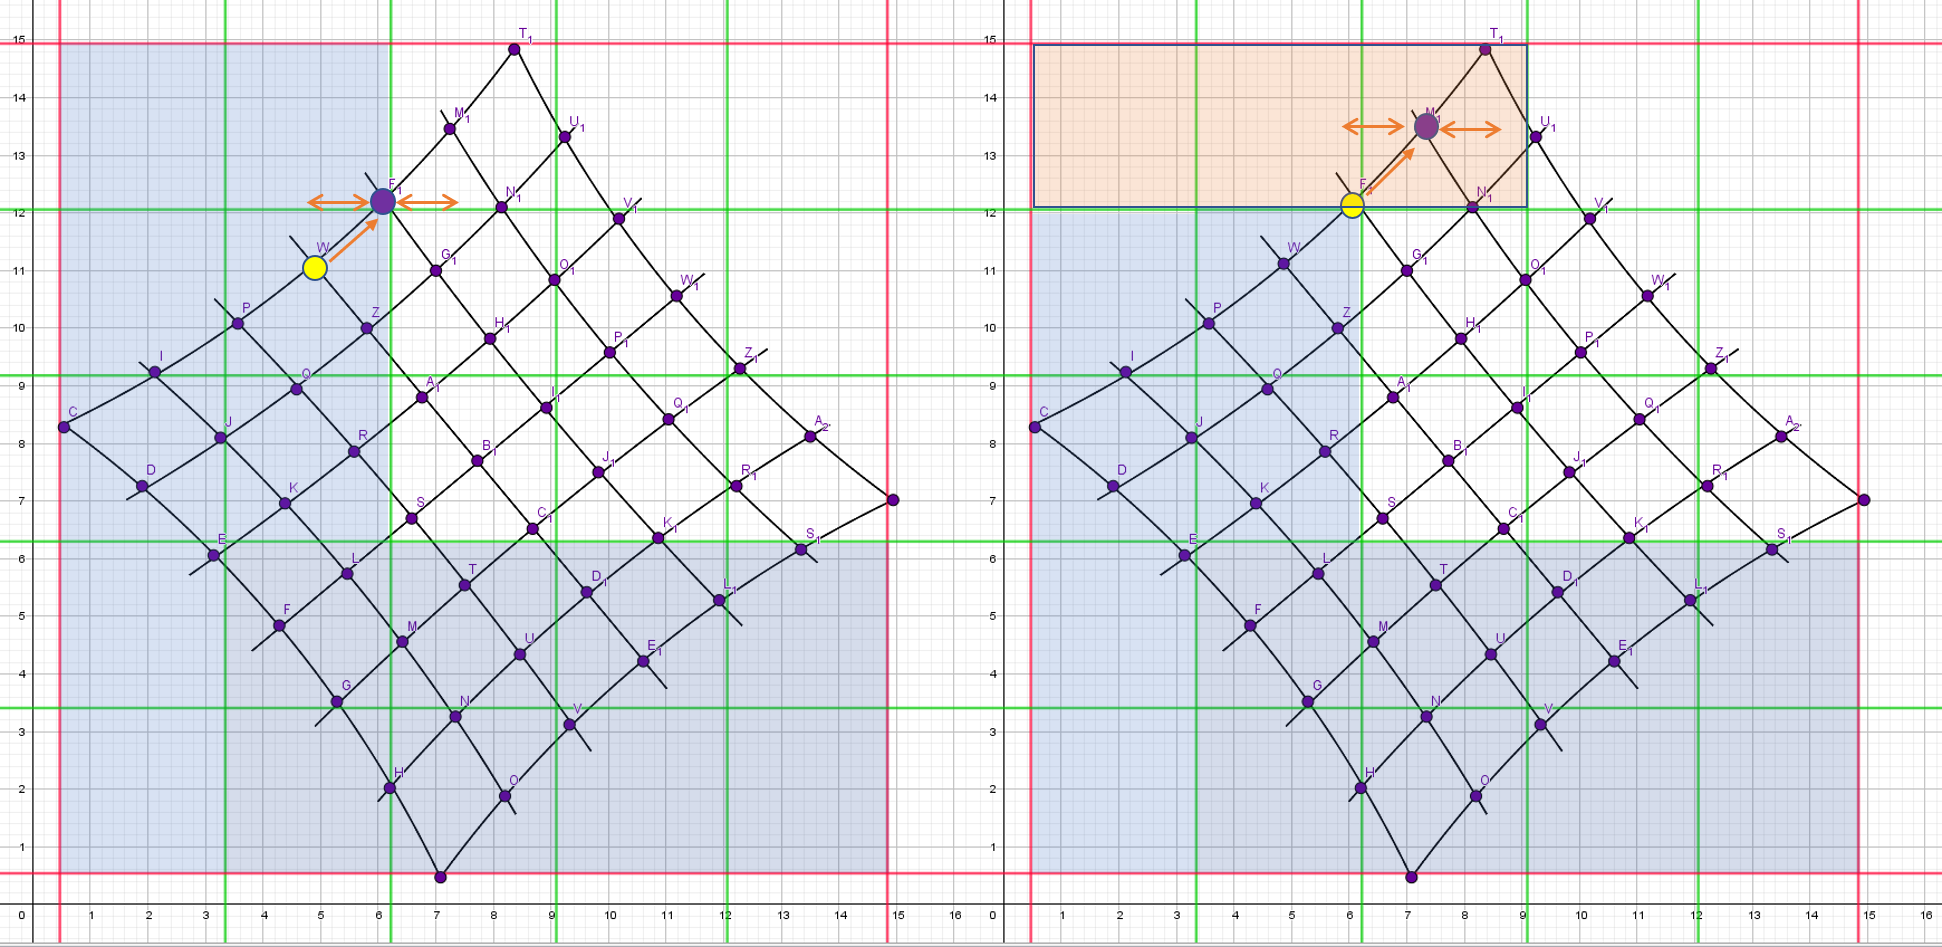
\includegraphics[width=1\linewidth]{images/VerzeichnetesSchachbrett_6.png}
	\captionof{figure}{Klassendiagramm}
\end{minipage}\\


\section{Extrembeispiele}
\label{sec:SchachAlgBeispiele}

In den folgenden Beispielen sieht man jeweils das Originalbild und ein Bild welches die durch den Algorithmus sortierten Punkte farbig ausgibt. Die grünen eingefärbten Punkte sind in den Bildern des Algorithmus die Nachbarn, welche sich in i-Richtung an der dritten Stelle befinden. Natürlich können auch andere Reihen oder auch einzelne Punkte abgefragt werden. 
\pagebreak

\begin{figure}[!htb]
	\minipage{0.48\textwidth}
	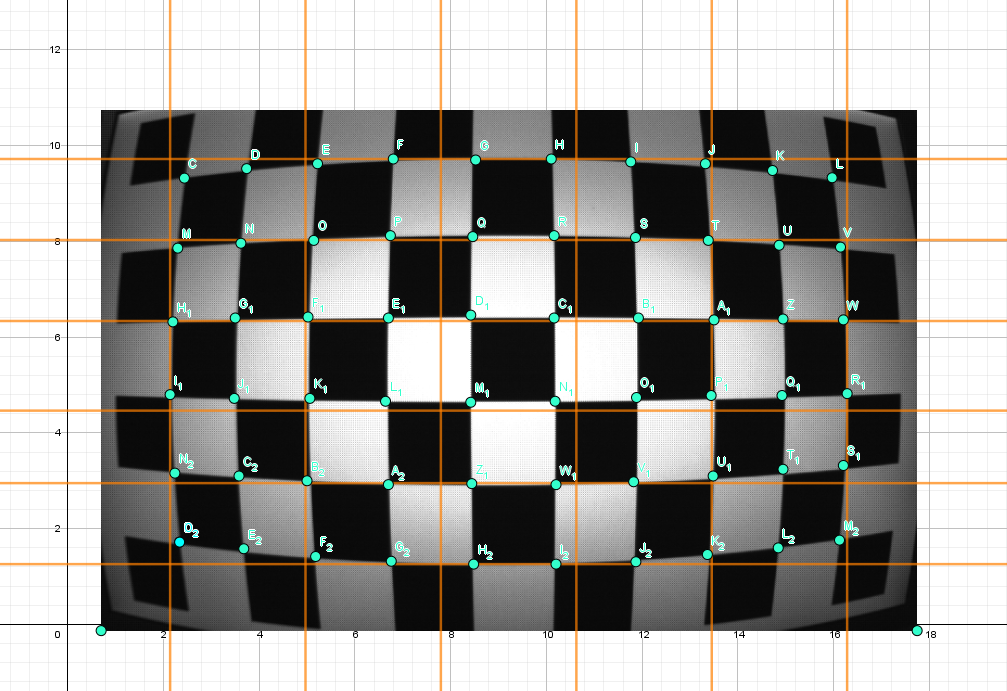
\includegraphics[width=\linewidth]{images/Tonnenverzeichnung.png}
	\caption{Bild eines Tonnenförmig verzeichneten Schachbretts}
	\label{fig:awesome_image1}
	\endminipage\hfill
	\minipage{0.48\textwidth}
	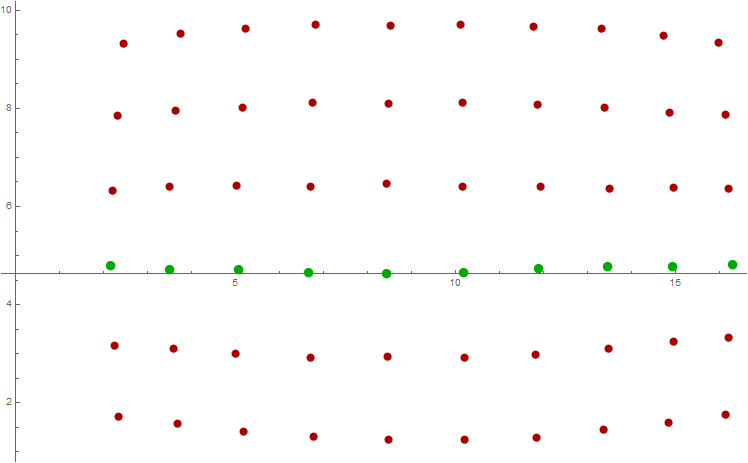
\includegraphics[width=\linewidth]{images/AlgTonnenverzeichnung.png}
	\caption{Algorithmisch detektierte Linie der dritten i-Reihe}
	\label{fig:awesome_image2}
	\endminipage\hfill
\end{figure}

\begin{figure}[!htb]
	\minipage{0.48\textwidth}
	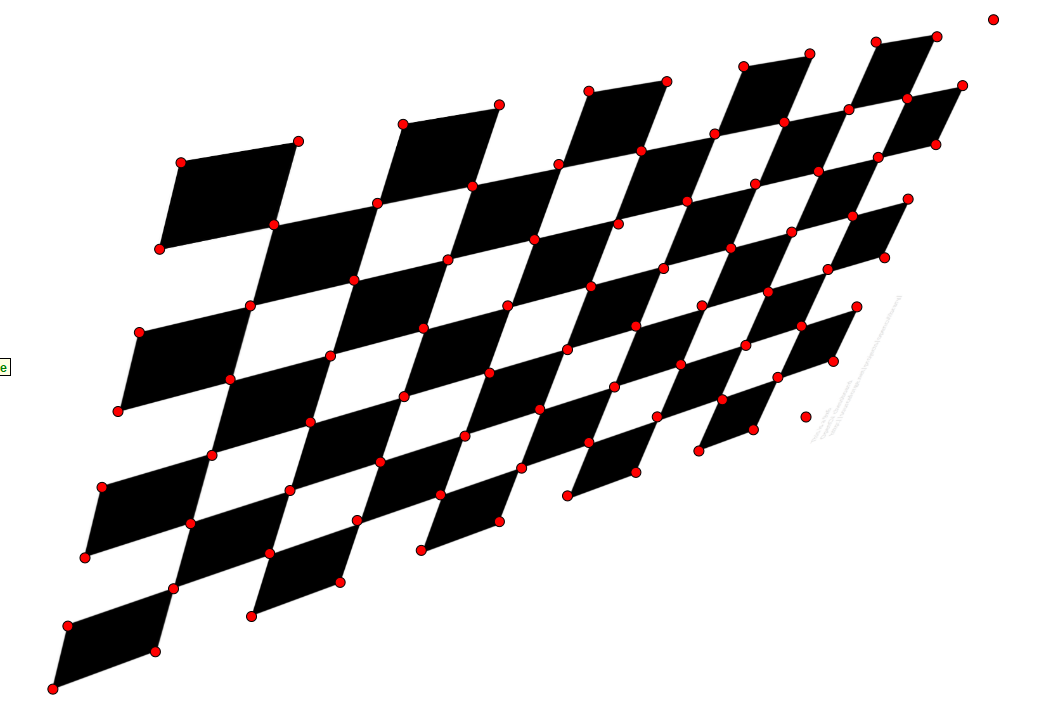
\includegraphics[width=\linewidth]{images/perspektivisch.png}
	\caption{Bild eines perspektivisch verzerrtem Schachbretts}
	\label{fig:awesome_image1}
	\endminipage\hfill
	\minipage{0.48\textwidth}
	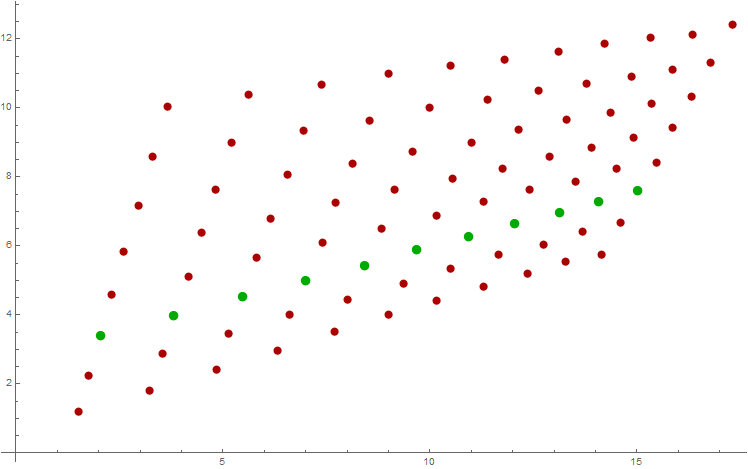
\includegraphics[width=\linewidth]{images/AlgPerspektifisch.png}
	\caption{Algorithmisch detektierte Linie der dritten i-Reihe}
	\label{fig:awesome_image2}
	\endminipage\hfill
\end{figure}


\begin{figure}[!htb]
	\minipage{0.48\textwidth}
	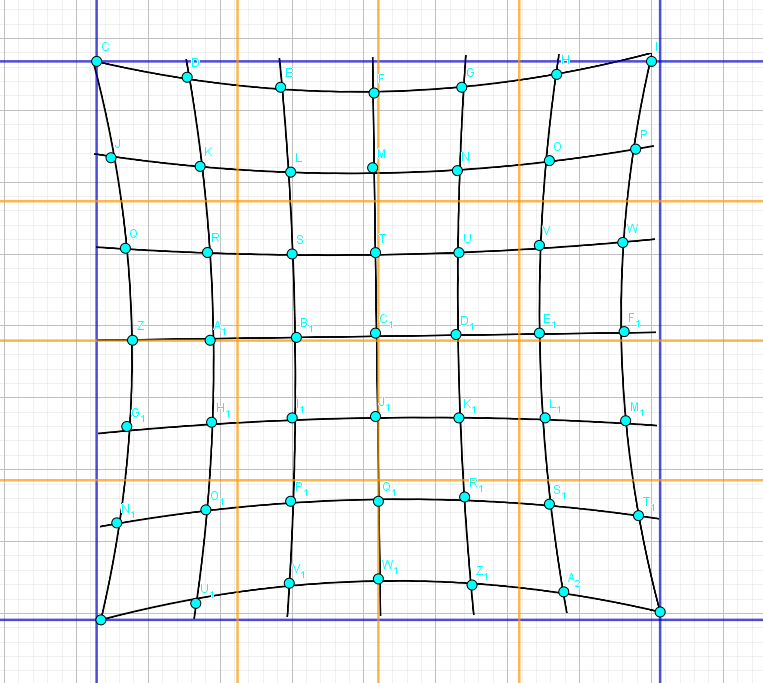
\includegraphics[width=\linewidth]{images/KissenVerzeichnung.png}
	\caption{Bild eines Kissenförmig verzeichnetem Schachbretts}
	\label{fig:awesome_image1}
	\endminipage\hfill
	\minipage{0.48\textwidth}
	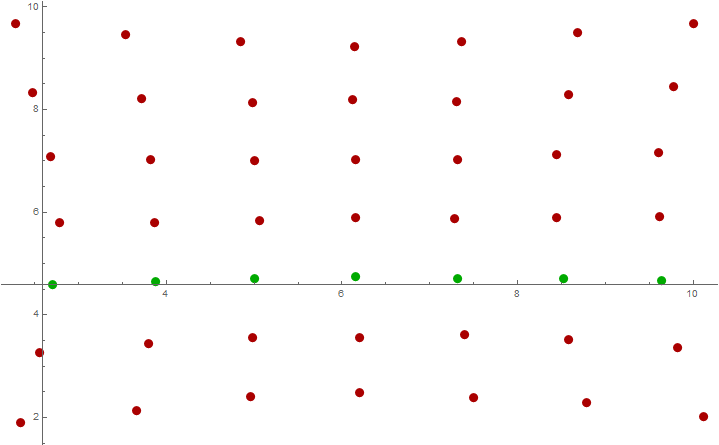
\includegraphics[width=\linewidth]{images/AlgKissen.png}
	\caption{Algorithmisch detektierte Linie der dritten i-Reihe}
	\label{fig:awesome_image2}
	\endminipage\hfill
\end{figure}

\begin{figure}[!htb]
	\minipage{0.48\textwidth}
	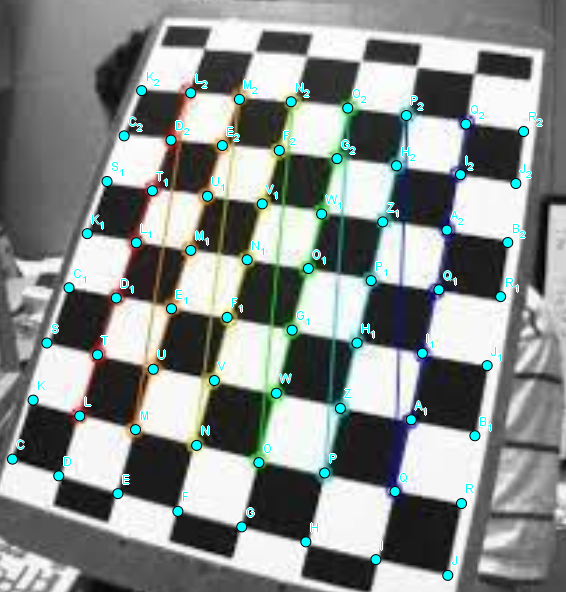
\includegraphics[width=\linewidth]{images/TonnePers.png}
	\caption{Bild eines Tonnenförmig verzeichnetem leicht perspektivisch verzerrtem Schachbretts(GRFIK AUSTAUSCHEN BILD IS KACKE)}
	\label{fig:awesome_image1}
	\endminipage\hfill
	\minipage{0.48\textwidth}
	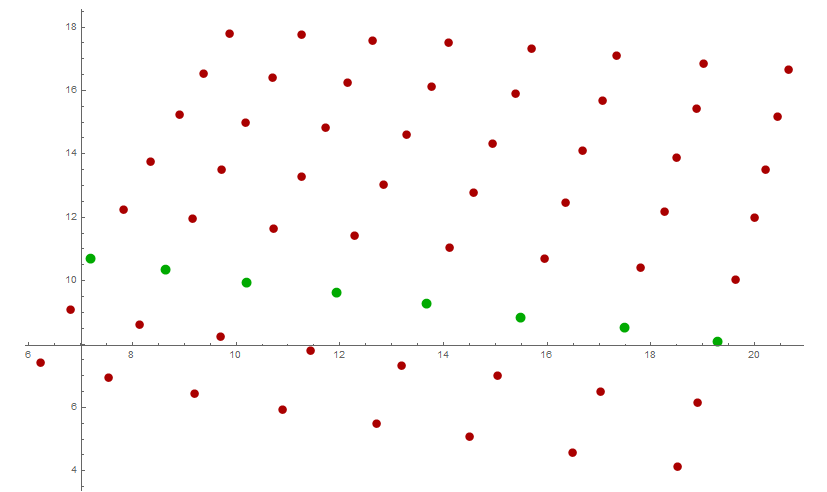
\includegraphics[width=\linewidth]{images/AlgTonnePers.png}
	\caption{Algorithmisch detektierte Linie der dritten i-Reihe}
	\label{fig:awesome_image2}
	\endminipage\hfill
\end{figure}

\begin{figure}[!htb]
	\minipage{0.48\textwidth}
	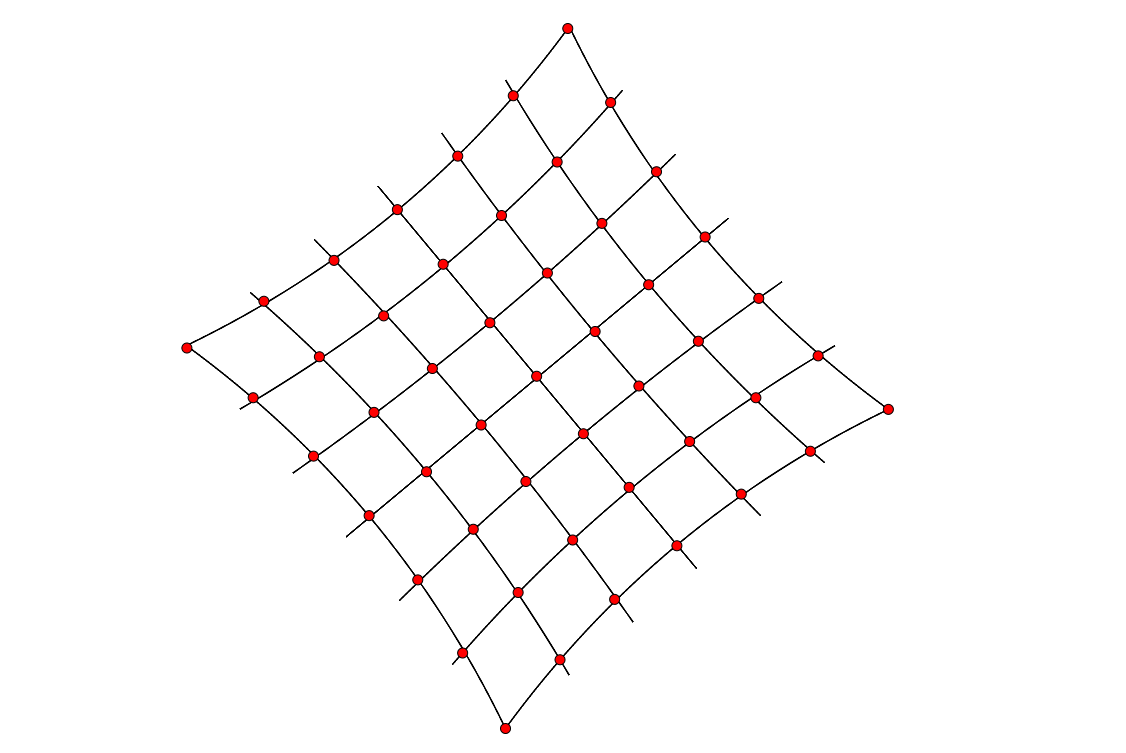
\includegraphics[width=\linewidth]{images/extrBsp.png}
	\caption{Bild eines Tonnenförmig verzeichnetem leicht perspektivisch verzerrtem Schachbretts}
	\label{fig:awesome_image1}
	\endminipage\hfill
	\minipage{0.48\textwidth}
	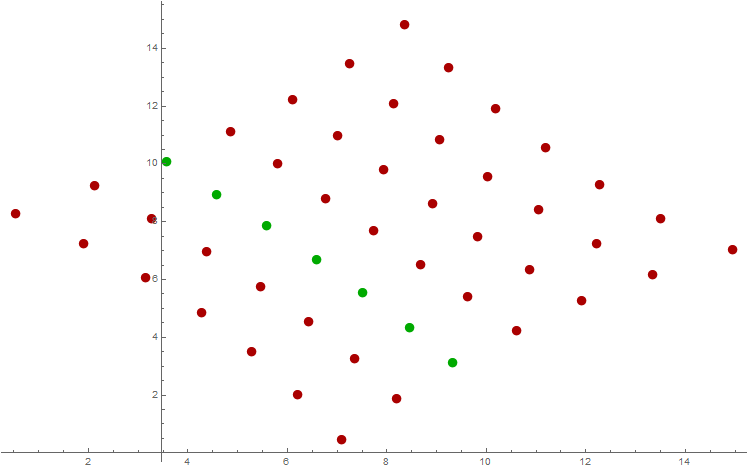
\includegraphics[width=\linewidth]{images/AlgExtrBsp.png}
	\caption{Algorithmisch detektierte Linie der dritten i-Reihe}
	\label{fig:awesome_image2}
	\endminipage\hfill
\end{figure}


\section{Modulübersicht}


\begin{minipage}{\linewidth}
	\centering
	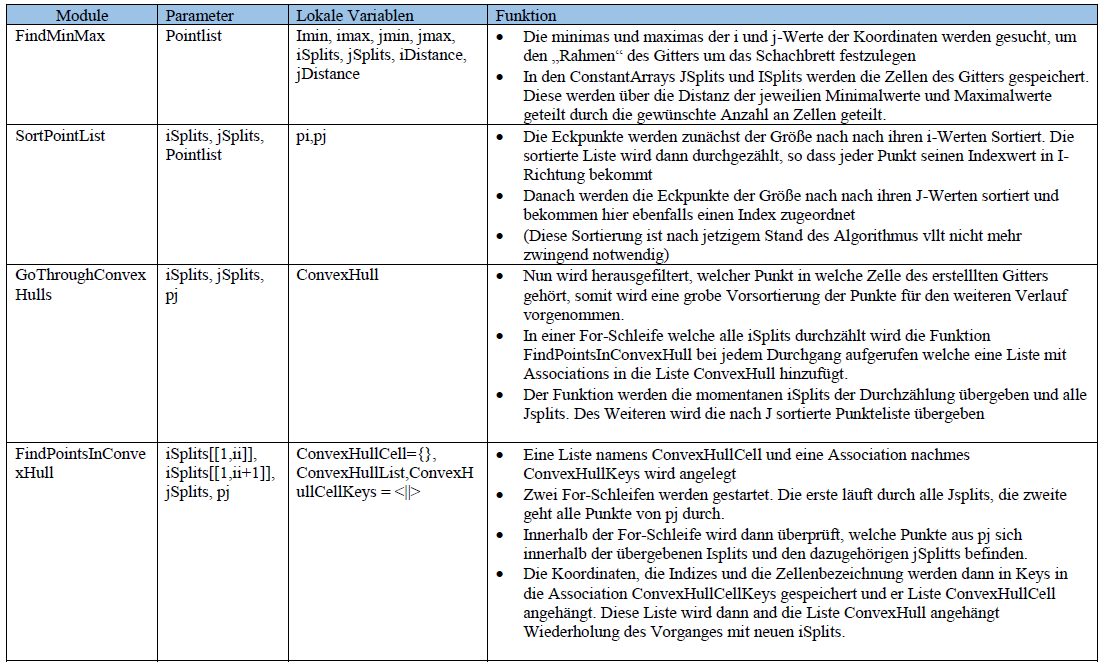
\includegraphics[width=1\linewidth]{images/KD1.png}
	\captionof{figure}{Klassendiagramm}
\end{minipage}
\begin{minipage}{\linewidth}
	\centering
	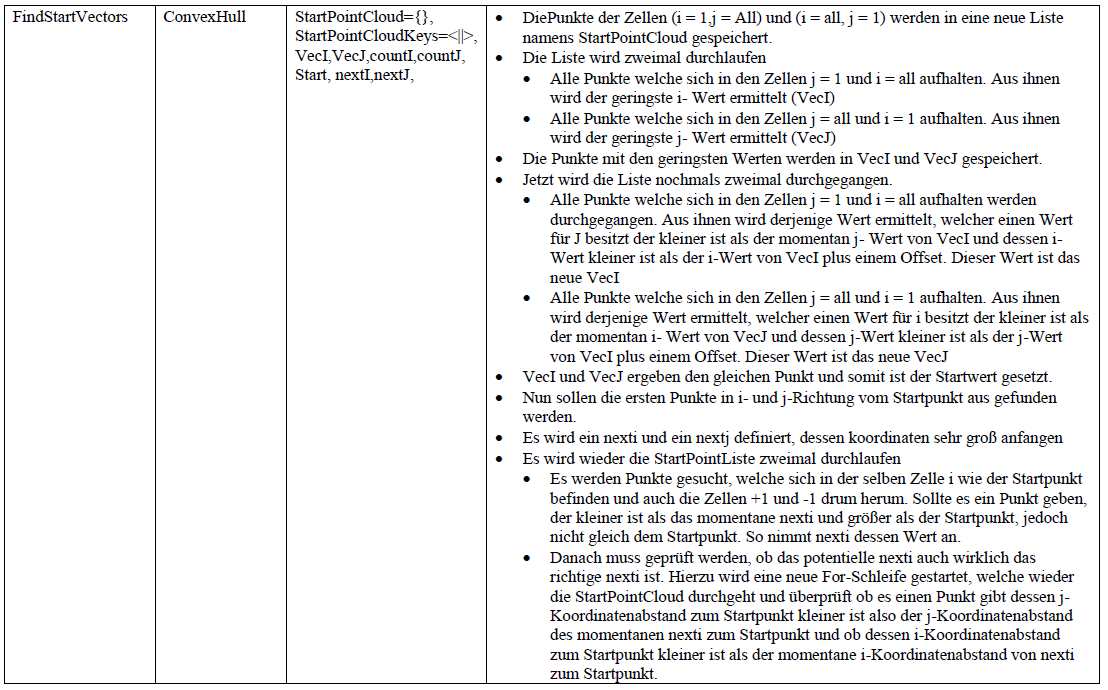
\includegraphics[width=1\linewidth]{images/KD2.png}
	\captionof{figure}{Klassendiagramm}
\end{minipage}
\begin{minipage}{\linewidth}
	\centering
	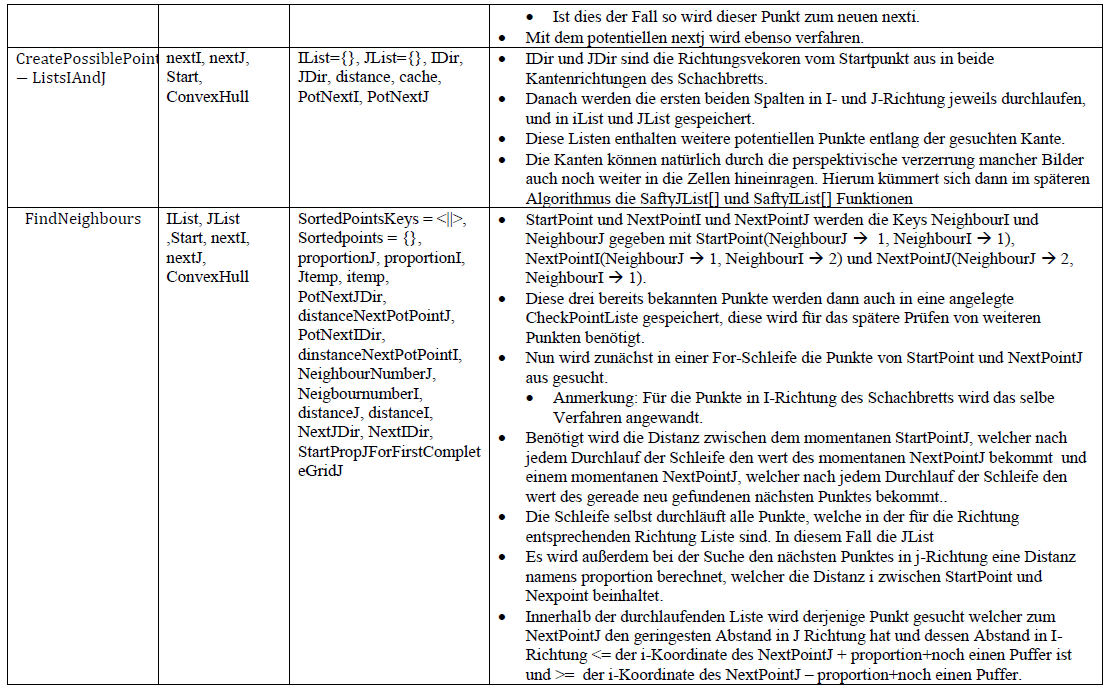
\includegraphics[width=1\linewidth]{images/KD3.png}
	\captionof{figure}{Klassendiagramm}
\end{minipage}
\begin{minipage}{\linewidth}
	\centering
	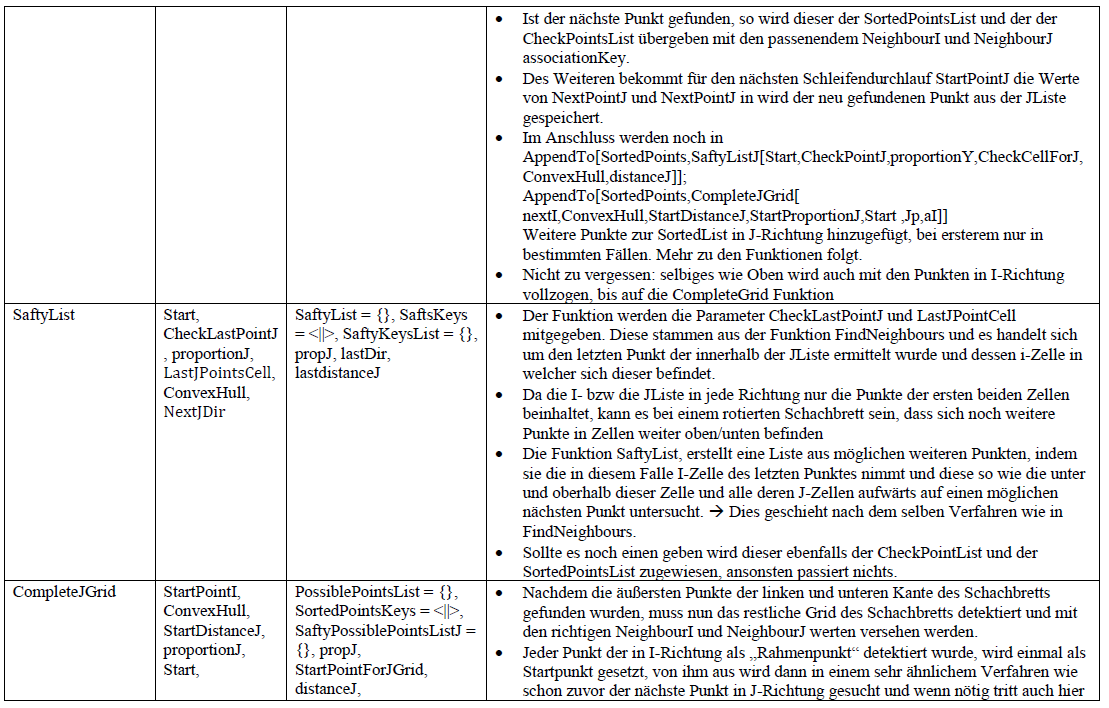
\includegraphics[width=1\linewidth]{images/KD4.png}
	\captionof{figure}{Klassendiagramm}
\end{minipage}
\begin{minipage}{\linewidth}
	\centering
	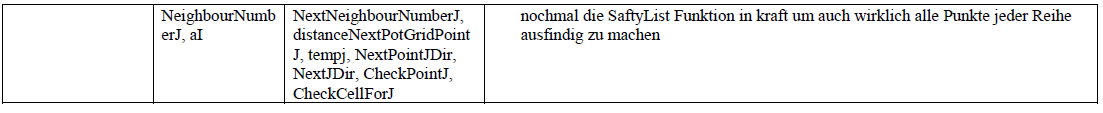
\includegraphics[width=1\linewidth]{images/KD5.png}
	\captionof{figure}{Klassendiagramm}
\end{minipage}\\







